\documentclass[11pt]{article}
\usepackage[margin=0.9in]{geometry}
\usepackage{amsmath,amssymb,bm}
\usepackage{fontspec}
\setmonofont{DejaVu Sans Mono}[Scale=0.78]
\usepackage{graphicx,booktabs,float,fancyvrb,xcolor,hyperref}
\hypersetup{colorlinks=true,linkcolor=blue,urlcolor=blue}
\setlength{\parskip}{4pt}\setlength{\parindent}{0pt}
\newcommand{\x}{\mathbf{x}}\newcommand{\z}{\mathbf{z}}\newcommand{\w}{\mathbf{w}}
\DeclareMathOperator*{\argmin}{arg\,min}\DeclareMathOperator*{\argmax}{arg\,max}

\title{EECE5644 Fall 2026 -- Assignment 2}
\author{David Abu}
\date{}
\begin{document}
\maketitle

\noindent All experiments were implemented in Python 3 (NumPy 2.5, SciPy 1.18, Matplotlib 3.11) with fixed random seeds, so every number below is reproducible from the code in the Appendix.

%=====================================================================
\section*{Question 1}

\subsection*{Data}
Each sample's label is drawn with $P(L{=}1)=0.4$; given $L=l$, one of the two equally weighted Gaussian components $g(\x|\mathbf m_{l1},C)$, $g(\x|\mathbf m_{l2},C)$ is chosen and $\x$ is drawn from it, with $C=\mathrm{diag}(0.75,1.25)$. Datasets $D^{20}_{train},D^{200}_{train},D^{2000}_{train},D^{10K}_{validate}$ were generated independently. The validation set contains $N_0=5949$, $N_1=4051$ samples.

\subsection*{Part 1: Theoretically optimal (min-P(error)) classifier}
With 0--1 loss, the minimum-risk rule is the MAP rule: decide $D=1$ iff $P(L{=}1|\x)>P(L{=}0|\x)$, i.e.\ the likelihood-ratio test
\[
\frac{p(\x|L{=}1)}{p(\x|L{=}0)}
=\frac{\tfrac12 g(\x|\mathbf m_{11},C)+\tfrac12 g(\x|\mathbf m_{12},C)}{\tfrac12 g(\x|\mathbf m_{01},C)+\tfrac12 g(\x|\mathbf m_{02},C)}
\;\underset{D=0}{\overset{D=1}{\gtrless}}\;\gamma^\ast=\frac{P(L{=}0)}{P(L{=}1)}=\frac{0.6}{0.4}=1.5 .
\]
The discriminant score used for the ROC is the log-likelihood ratio $s(\x)=\ln p(\x|L{=}1)-\ln p(\x|L{=}0)$, thresholded at $\ln\gamma$. Sweeping $\ln\gamma$ over all observed score values gives the ROC curve ($P_{FA}=P(D{=}1|L{=}0)$ vs.\ $P_D=P(D{=}1|L{=}1)$); for each threshold the empirical error is
\[P(\text{error})=P_{FA}\,P(L{=}0)+(1-P_D)\,P(L{=}1)\]
with priors estimated from the validation labels.

\begin{table}[H]\centering
\begin{tabular}{lcc}\toprule
 & $L=0$ & $L=1$\\\midrule
$D=0$ & 5011 & 1855\\
$D=1$ & 938 & 2196\\\bottomrule
\end{tabular}
\caption{Decision/label counts of the optimal classifier ($\gamma^\ast=1.5$) on $D^{10K}_{validate}$.}
\end{table}

\textbf{Estimated min-P(error)} $=\dfrac{938+1855}{10000}=\mathbf{0.2793}$ \;($P_{FA}=0.1577$, $P_D=0.5421$). The empirically best threshold on the ROC is $\ln\gamma=0.433$ (vs.\ theoretical $0.405$) with $P(\text{error})=0.2779$; the small gap is finite-sample noise, confirming the theory.

\begin{figure}[H]\centering
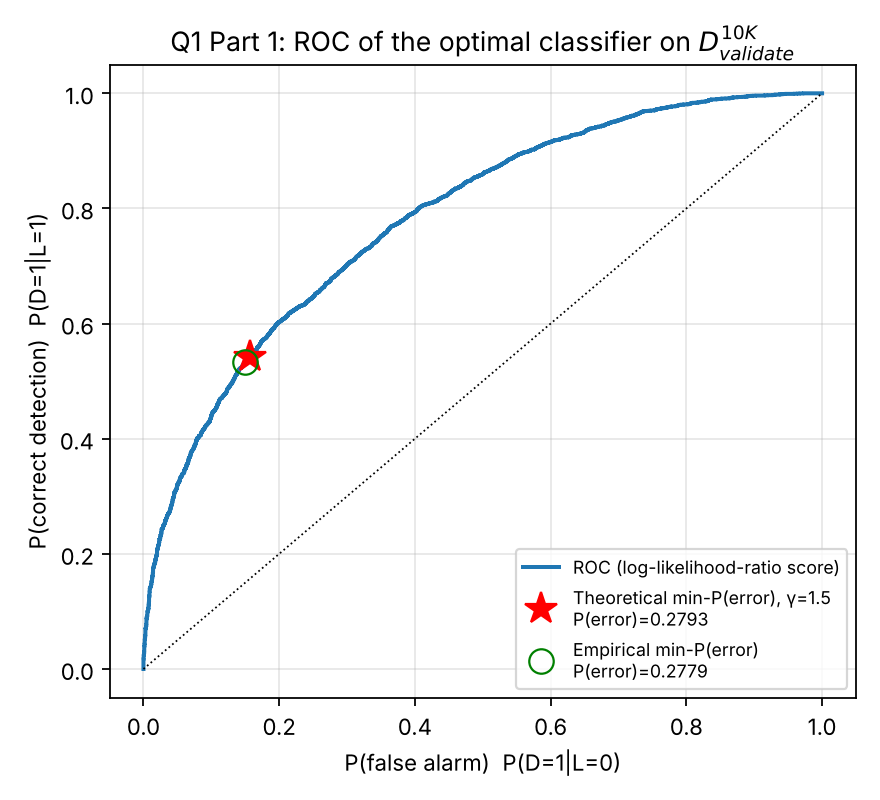
\includegraphics[width=0.46\linewidth]{figs/q1_roc.png}\hfill
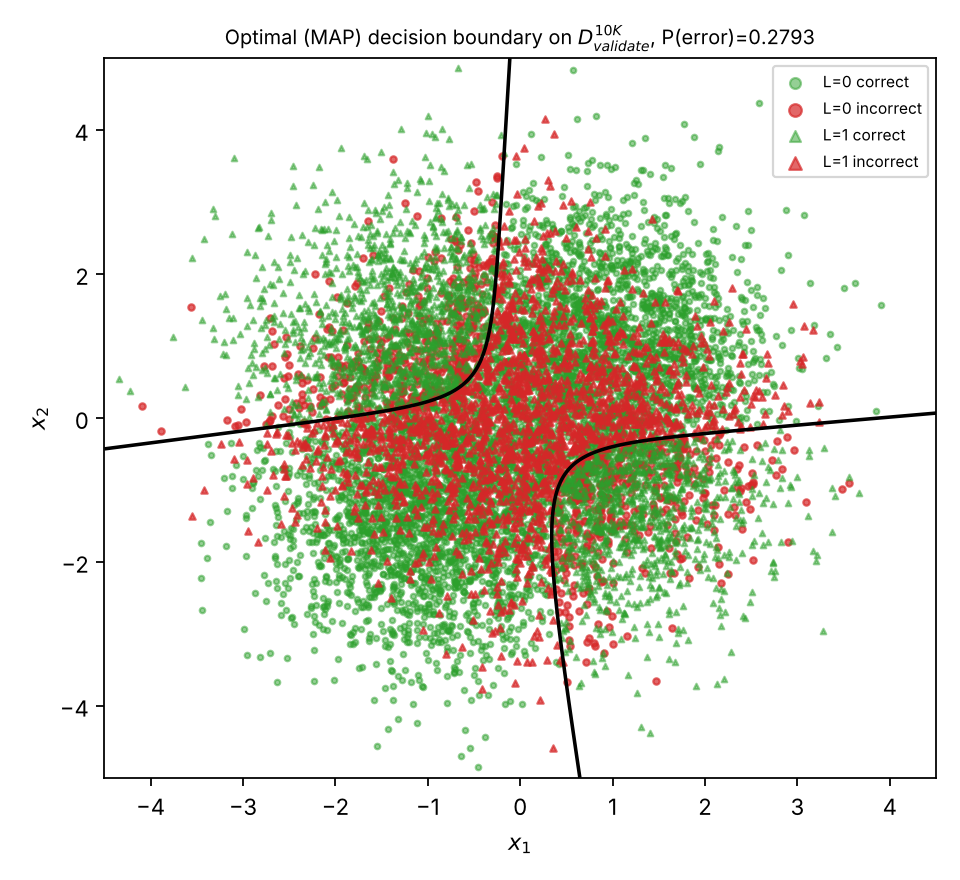
\includegraphics[width=0.5\linewidth]{figs/q1_opt_boundary.png}
\caption{Left: ROC of the log-likelihood-ratio score with the theoretical min-P(error) operating point (red star) and the empirical optimum (green circle). Right: optimal decision boundary on $D^{10K}_{validate}$ (green = correct, red = misclassified).}
\end{figure}

The boundary is a pair of hyperbola-like curves: class 0 occupies the 3rd and 1st quadrants and class 1 the 2nd and 4th (an XOR-like arrangement), so no single line can separate them.

\subsection*{Part 2: Logistic approximations trained by maximum likelihood}
Let $h(\x,\w)=\sigma(\w^T\z(\x))$, $\sigma(a)=1/(1+e^{-a})$, model $P(L{=}1|\x)$, with $\z(\x)=[1,x_1,x_2]^T$ (linear) or $\z(\x)=[1,x_1,x_2,x_1^2,x_1x_2,x_2^2]^T$ (quadratic). For iid training data $\{(\x_n,l_n)\}_{n=1}^N$ the likelihood is $\prod_n h_n^{l_n}(1-h_n)^{1-l_n}$, so the ML problem is
\[
\hat\w_{ML}=\argmin_\w \; -\frac1N\sum_{n=1}^N\Big[l_n\ln h(\x_n,\w)+(1-l_n)\ln\big(1-h(\x_n,\w)\big)\Big],
\qquad \nabla_\w=\frac1N\sum_n\big(h(\x_n,\w)-l_n\big)\z(\x_n).
\]
The objective is convex in $\w$; it was minimized with BFGS (\texttt{scipy.optimize.minimize}) using the analytic gradient, starting from $\w=\mathbf 0$ (implemented stably as $\ln(1+e^{a})-la$, $a=\w^T\z$).

\textbf{Classification rule.} Since $h(\x,\hat\w)\approx P(L{=}1|\x)$, the min-P(error) (MAP) rule becomes: decide $D=1$ iff $h(\x,\hat\w)\ge 0.5$, equivalently $\hat\w^T\z(\x)\ge 0$. (The priors are already absorbed into the learned bias term, because the training labels are sampled with the true priors.)

\begin{table}[H]\centering
\resizebox{\linewidth}{!}{\begin{tabular}{lcccc}\toprule
Model & $N_{train}$ & train P(error) & \textbf{validation P(error)} & $\hat\w_{ML}$\\\midrule
logistic-linear & 20 & 0.250 & \textbf{0.4198} & $[-1.145,\,0.357,\,0.263]$\\
logistic-linear & 200 & 0.410 & \textbf{0.3793} & $[-0.286,\,-0.088,\,0.232]$\\
logistic-linear & 2000 & 0.422 & \textbf{0.4074} & $[-0.337,\,0.013,\,0.110]$\\\midrule
logistic-quadratic & 20 & 0.150 & \textbf{0.3410} & $[-8.38,\,19.06,\,16.22,\,-11.85,\,-23.58,\,-5.67]$\\
logistic-quadratic & 200 & 0.330 & \textbf{0.2851} & $[-0.335,\,-0.018,\,0.183,\,0.067,\,-0.511,\,-0.010]$\\
logistic-quadratic & 2000 & 0.279 & \textbf{0.2795} & $[-0.368,\,0.000,\,0.119,\,0.065,\,-0.869,\,-0.050]$\\\midrule
Optimal (Part 1) & -- & -- & \textbf{0.2793} & --\\\bottomrule
\end{tabular}}
\caption{P(error) estimated by counting decisions on $D^{10K}_{validate}$. For reference, always deciding $D=0$ gives $\approx0.405$.}
\end{table}

\begin{figure}[H]\centering
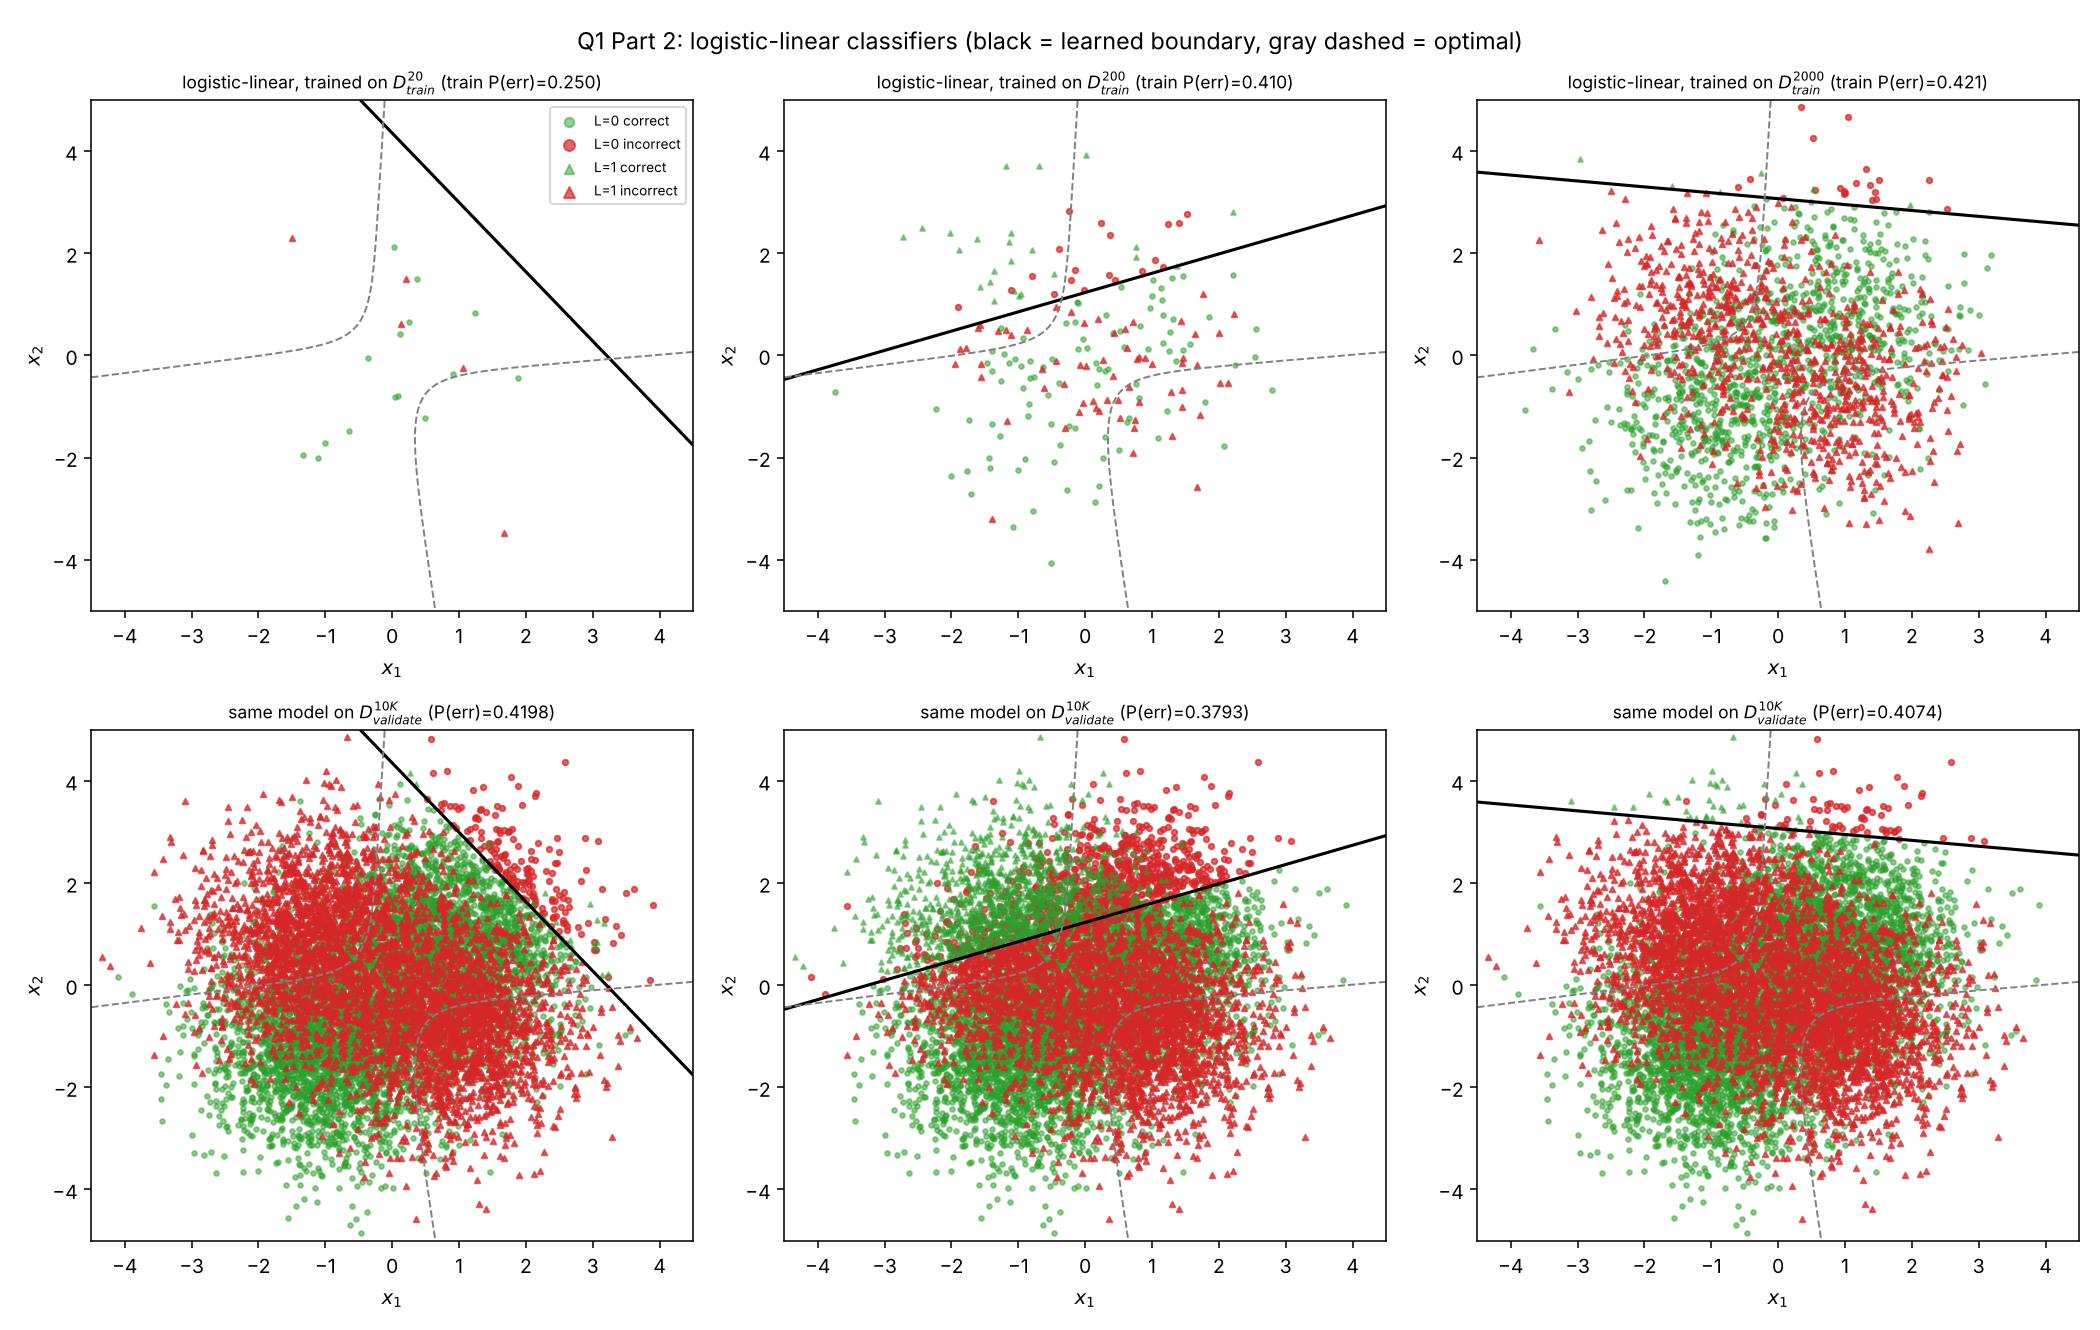
\includegraphics[width=\linewidth]{figs/q1_logistic_linear.png}
\caption{Logistic-linear classifiers. Top: training sets; bottom: validation set. Black = learned boundary, gray dashed = optimal boundary.}
\end{figure}
\begin{figure}[H]\centering
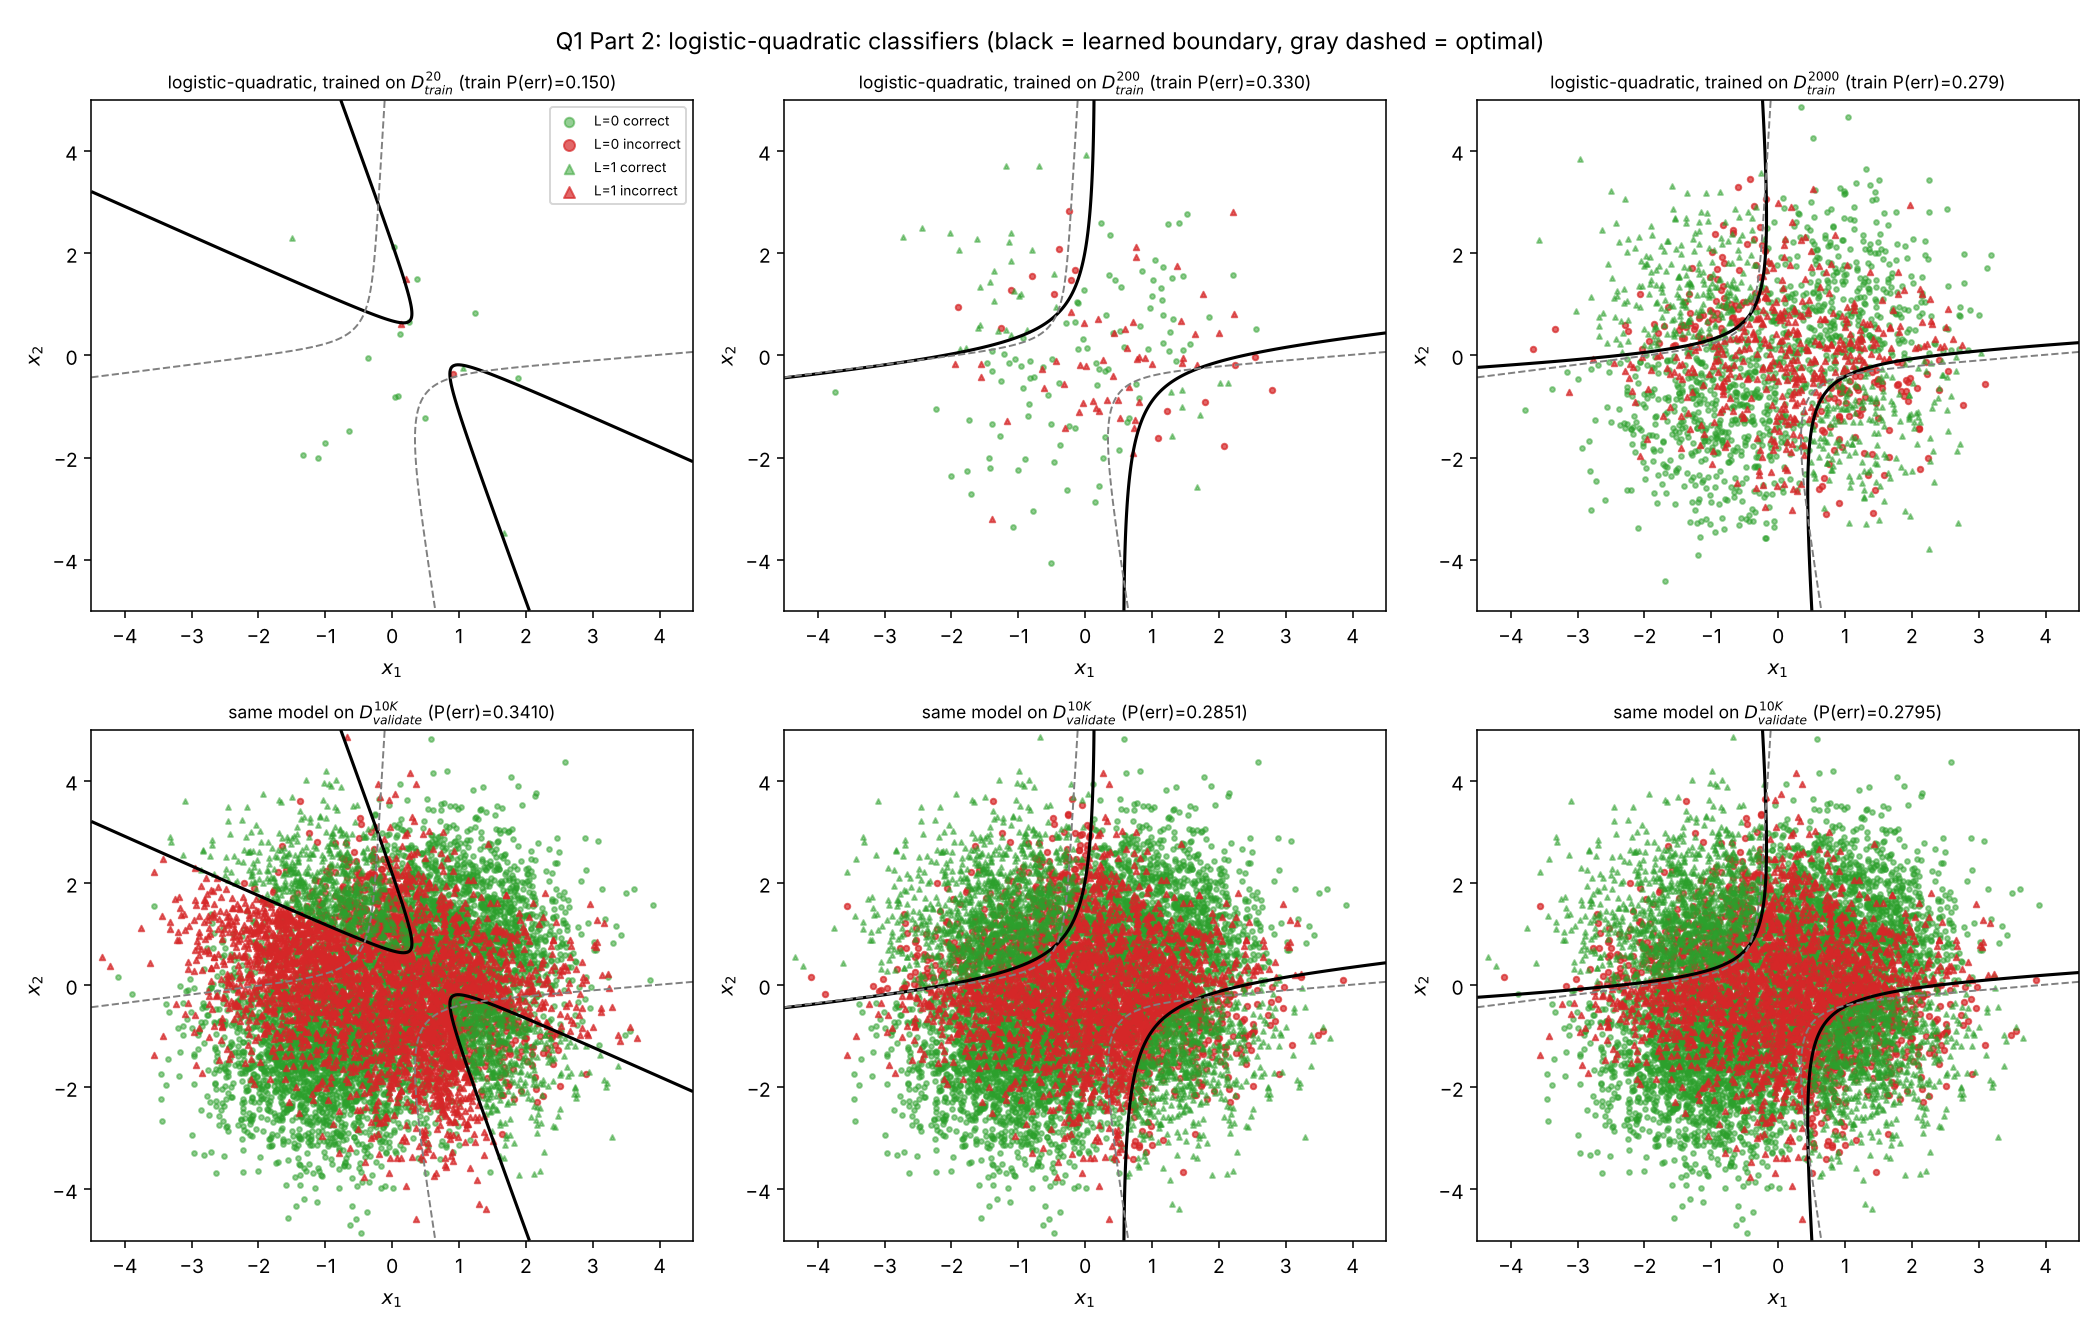
\includegraphics[width=\linewidth]{figs/q1_logistic_quadratic.png}
\caption{Logistic-quadratic classifiers, same layout.}
\end{figure}
\begin{figure}[H]\centering
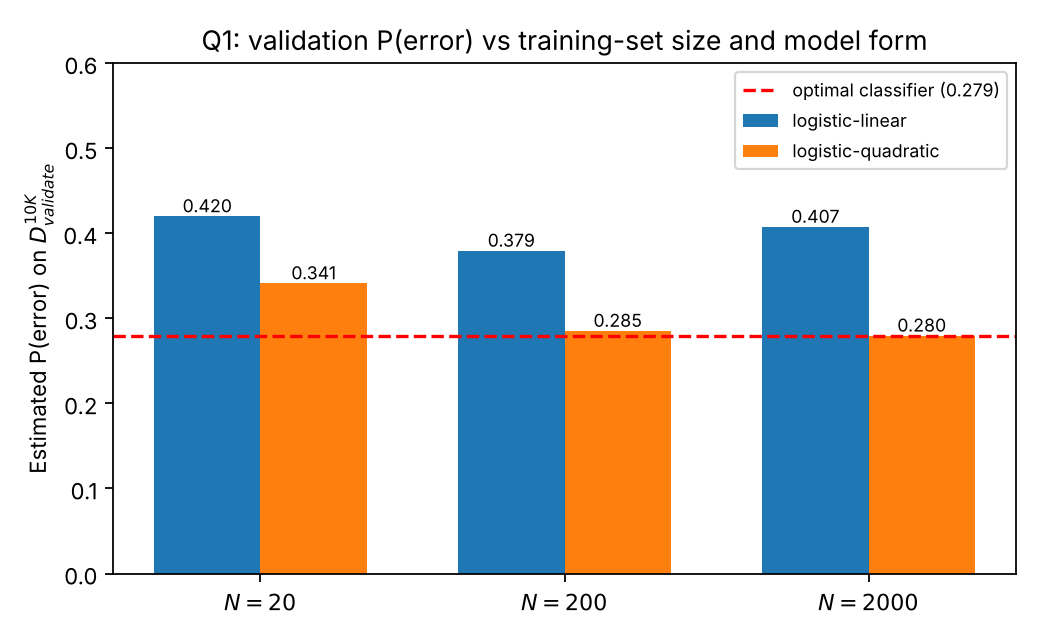
\includegraphics[width=0.6\linewidth]{figs/q1_summary.png}
\caption{Validation P(error) vs.\ training size and model form; red dashed = optimal classifier.}
\end{figure}

\subsection*{Discussion}
\begin{itemize}
\item \textbf{Function form dominates.} The Bayes boundary is XOR-like (opposite quadrants share a class), so a linear boundary cannot represent it. Even with 2000 samples the logistic-linear model reaches only 0.41, essentially no better than always predicting the majority class (0.405); its weights on $x_1,x_2$ are near zero because the classes have nearly identical marginal means. More data cannot fix this bias.
\item \textbf{The quadratic model contains the right structure.} The cross term $x_1x_2$ (weight $\approx-0.87$ at $N{=}2000$) is negative in the class-0 quadrants and positive in the class-1 quadrants, which is exactly the XOR pattern. With $N=2000$ it attains 0.2795, statistically indistinguishable from the optimal 0.2793, and its boundary overlays the optimal one (Fig.\ above). The true posterior is not exactly logistic-quadratic (it is a ratio of Gaussian mixtures), but a quadratic log-odds is an excellent approximation where the data lie.
\item \textbf{Sample size controls variance/overfitting.} With $N=20$ the quadratic model nearly separates the training data (train error 0.15) and its weights blow up ($|w|\sim 20$), giving a distorted boundary and validation error 0.34. With $N=200$ the estimate stabilizes (0.285) and with $N=2000$ it converges to the Bayes boundary. The linear $N=20$ model also shows the optimism of training error (0.25 train vs.\ 0.42 validation).
\item \textbf{Relation to Part 1.} The Bayes (optimal) error is a lower bound on the \emph{expected} (population) P(error) of any classifier, not on every finite-sample error count: on a particular validation set a fitted classifier can score marginally below the optimal classifier's empirical error without contradicting theory. Here every trained classifier happens to score at or above 0.2793, and only a model flexible enough to represent the XOR structure, trained on enough data, approaches it.
\end{itemize}

%=====================================================================
\section*{Question 2}

\subsection*{Model and derivations}
Let $\z(\x)\in\mathbb R^{10}$ collect all monomials of $\x=[x_1,x_2]^T$ of total degree $\le3$:
\[\z(\x)=[1,x_1,x_2,x_1^2,x_1x_2,x_2^2,x_1^3,x_1^2x_2,x_1x_2^2,x_2^3]^T,\]so $c(\x,\w)=\w^T\z(\x)$ and $y_n=\w^T\z_n+v_n$, $v_n\sim\mathcal N(0,\sigma^2)$ iid. Stack $Z=[\z_1,\dots,\z_N]^T\in\mathbb R^{N\times10}$, $\mathbf y=[y_1,\dots,y_N]^T$.

\textbf{ML.} $p(D|\w)=\prod_{n}(2\pi\sigma^2)^{-1/2}\exp\!\big(-\tfrac{(y_n-\w^T\z_n)^2}{2\sigma^2}\big)$, so
\[
\ln p(D|\w)=-\frac{N}{2}\ln(2\pi\sigma^2)-\frac{1}{2\sigma^2}\|\mathbf y-Z\w\|^2
\;\Rightarrow\;
\hat\w_{ML}=\argmin_\w\|\mathbf y-Z\w\|^2 .
\]
Setting $\nabla_\w=-2Z^T(\mathbf y-Z\w)=0$:
\[
\boxed{\hat\w_{ML}=(Z^TZ)^{-1}Z^T\mathbf y=\Big(\sum_n\z_n\z_n^T\Big)^{-1}\sum_n\z_n y_n .}
\]

\textbf{MAP.} With prior $\w\sim\mathcal N(\mathbf 0,\gamma I)$, $\ln p(\w)=-\frac{1}{2\gamma}\|\w\|^2+\text{const}$, and
\[
\hat\w_{MAP}=\argmax_\w\big[\ln p(D|\w)+\ln p(\w)\big]=\argmin_\w\Big[\frac{1}{\sigma^2}\|\mathbf y-Z\w\|^2+\frac1\gamma\|\w\|^2\Big].
\]
Setting the gradient $-\tfrac{2}{\sigma^2}Z^T(\mathbf y-Z\w)+\tfrac2\gamma\w$ to zero:
\[
\boxed{\hat\w_{MAP}=\Big(Z^TZ+\frac{\sigma^2}{\gamma}I\Big)^{-1}Z^T\mathbf y=\Big(\sum_n\z_n\z_n^T+\frac{\sigma^2}{\gamma}I\Big)^{-1}\sum_n\z_n y_n .}
\]
This is ridge regression with $\lambda=\sigma^2/\gamma$. \textbf{Relation to ML:} as $\gamma\to\infty$ (uninformative prior) $\lambda\to0$ and $\hat\w_{MAP}\to\hat\w_{ML}$; as $\gamma\to0$ the prior dominates and $\hat\w_{MAP}\to\mathbf 0$. For finite $\gamma$ the MAP estimate is the ML estimate shrunk toward zero: in the eigenbasis of $Z^TZ$ (eigenvalues $\mu_j$) each component is scaled by $\mu_j/(\mu_j+\lambda)$.

Since $\sigma^2$ is not given, a working residual-variance estimate from the ML fit was used, $\hat\sigma^2=\|\mathbf y-Z\hat\w_{ML}\|^2/(N-10)=3.636$. This would be unbiased if the data truly followed the cubic-plus-constant-variance-Gaussian model; the supplied mixture generator does not satisfy that model exactly, so it is a documented working choice rather than an unbiased estimate. Only the ratio $\lambda=\sigma^2/\gamma$ matters, so a different $\hat\sigma^2$ simply shifts the $\gamma$ axis.

\subsection*{Experiments}
Data were produced by the course-provided \texttt{hw2q2.py} generator ($N_{train}=100$, $N_{validate}=1000$; generator logic copied unchanged, with plotting removed and a fixed seed). $\gamma$ was swept over 161 log-spaced values in $[10^{-10},10^{6}]$ ($m=10$, $n=6$); every model was evaluated by the average squared error on the validation set, $\frac1{N_v}\sum_n(y_n-\hat\w^T\z(\x_n))^2$.

\begin{figure}[H]\centering
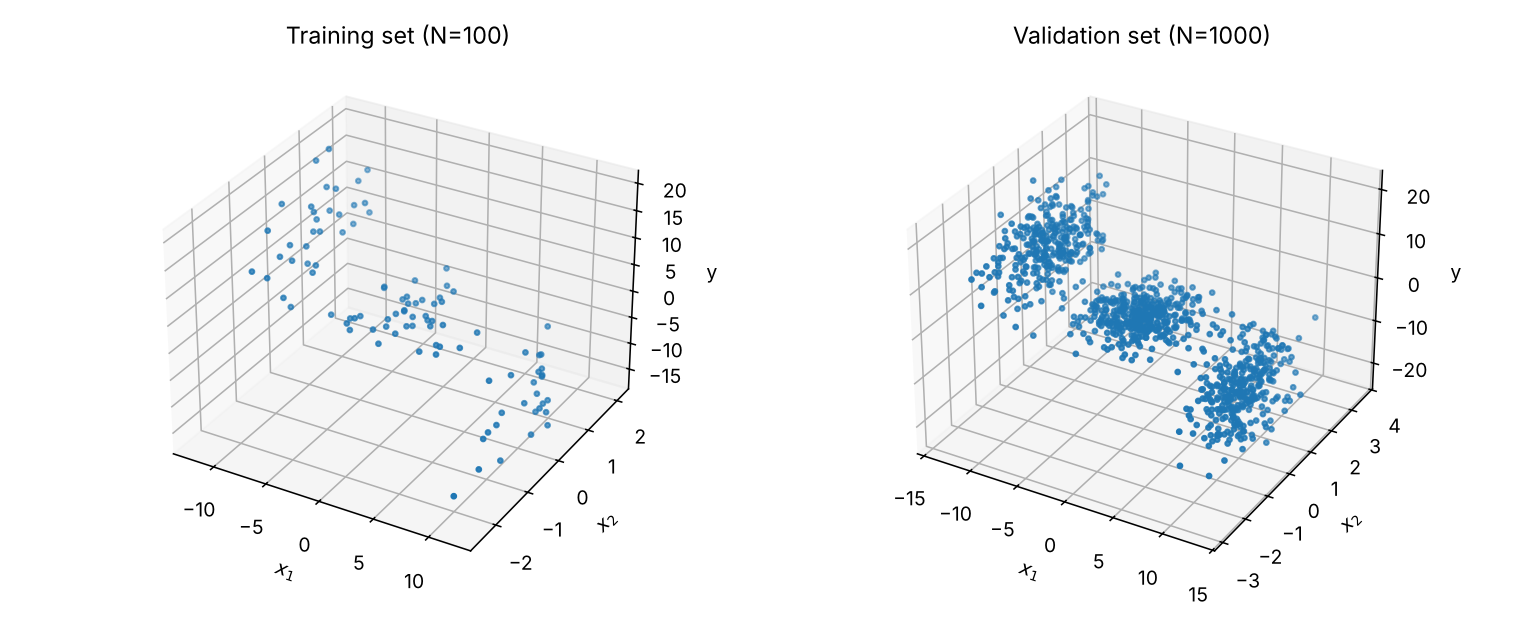
\includegraphics[width=0.85\linewidth]{figs/q2_data.png}
\caption{Training and validation data from the provided generator.}
\end{figure}

\textbf{ML:} training MSE $=3.272$, \textbf{validation MSE $=5.455$}.\\
$\hat\w_{ML}=[0.128,\,0.172,\,0.167,\,-0.0024,\,-0.0205,\,0.0733,\,-0.0108,\,0.0110,\,-0.0247,\,-0.470]$.

\begin{table}[H]\centering
\begin{tabular}{rccc}\toprule
$\gamma$ & validation MSE & $\|\hat\w_{MAP}\|$ & $\|\hat\w_{MAP}-\hat\w_{ML}\|$\\\midrule
$10^{-10}$ & 72.07 & 0.0000 & 0.549\\
$10^{-8}$ & 52.72 & 0.0015 & 0.549\\
$10^{-6}$ & 4.719 & 0.0089 & 0.549\\
$\mathbf{7.9\times10^{-6}}$ (best) & \textbf{4.427} & 0.0094 & 0.549\\
$10^{-4}$ & 4.504 & 0.0120 & 0.548\\
$10^{-2}$ & 4.703 & 0.107 & 0.468\\
$10^{0}$ & 5.294 & 0.501 & 0.069\\
$10^{2}$ & 5.453 & 0.549 & 0.0009\\
$10^{4},10^{6}$ & 5.455 & 0.549 & 0.0000\\\bottomrule
\end{tabular}
\caption{MAP results versus $\gamma$ (ML: validation MSE 5.455, $\|\hat\w_{ML}\|=0.549$).}
\end{table}

\begin{figure}[H]\centering
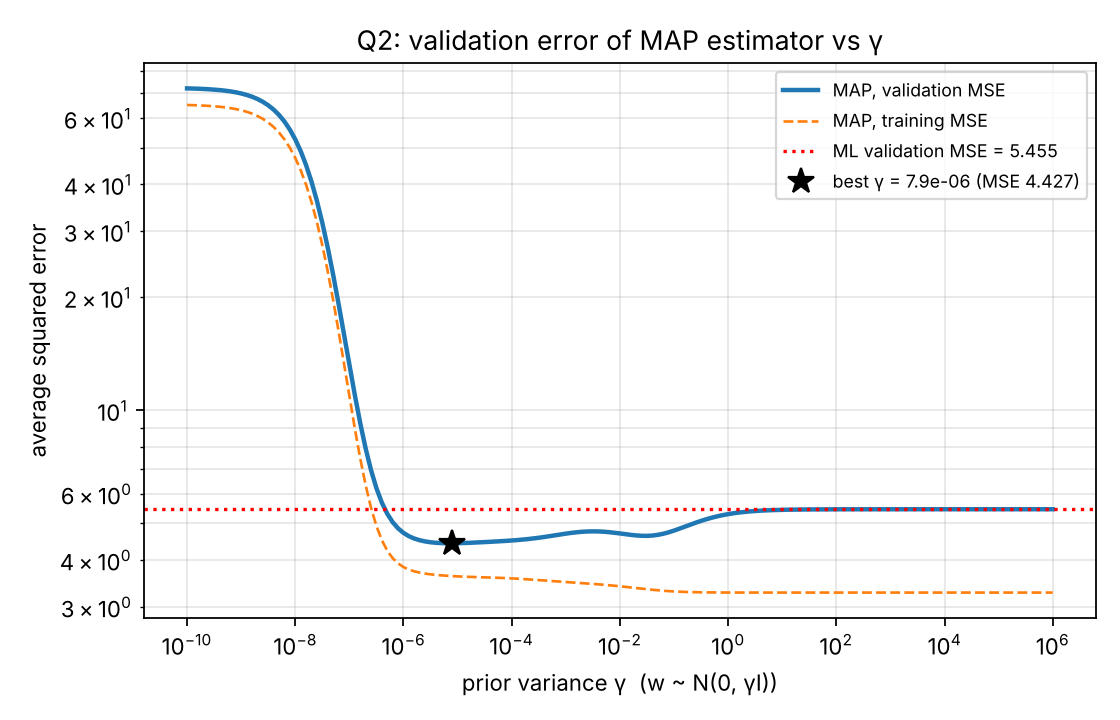
\includegraphics[width=0.49\linewidth]{figs/q2_mse_vs_gamma.png}\hfill
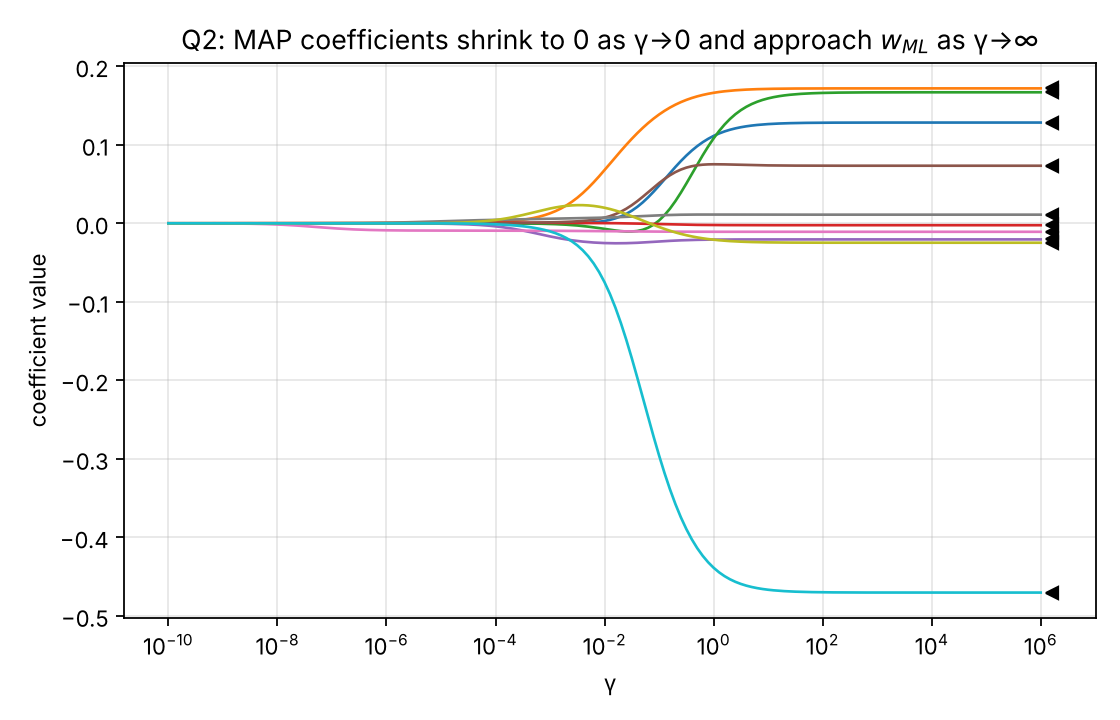
\includegraphics[width=0.49\linewidth]{figs/q2_coeff_path.png}
\caption{Left: training/validation MSE of the MAP estimator vs.\ $\gamma$ with the ML level (red). Right: MAP coefficients vs.\ $\gamma$; black triangles mark $\hat\w_{ML}$.}
\end{figure}

To check that the trend is not specific to one random draw, the whole experiment was repeated on 100 independent train/validation draws:

\begin{figure}[H]\centering
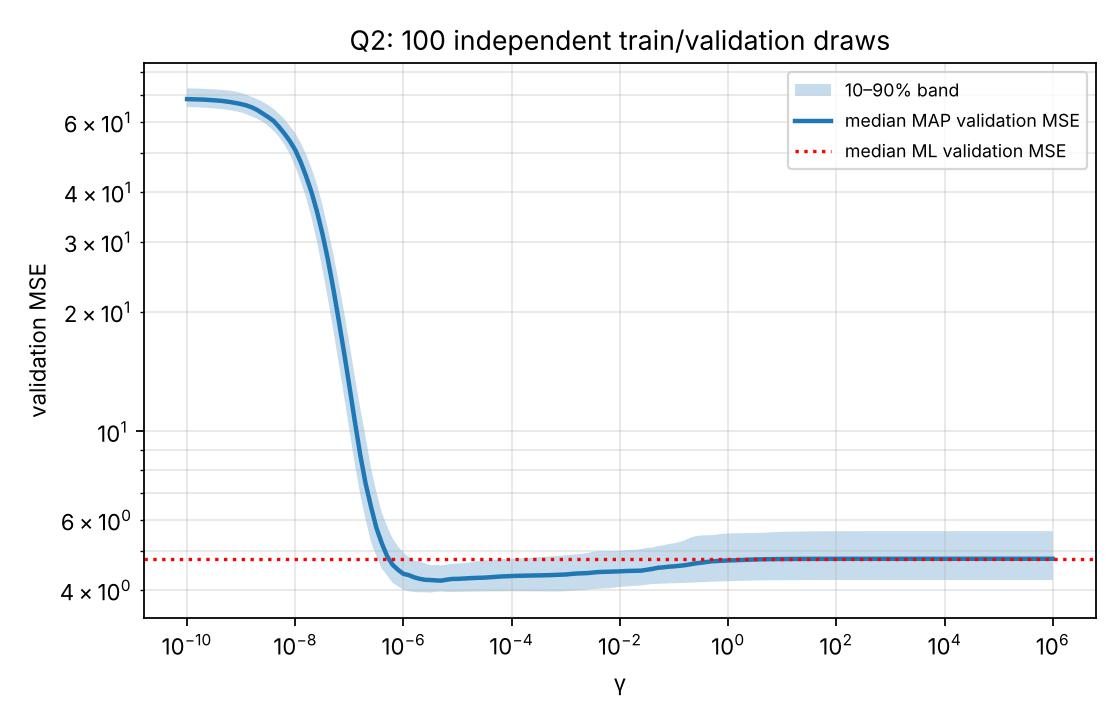
\includegraphics[width=0.6\linewidth]{figs/q2_mse_trials.png}
\caption{Median and 10--90\% band of MAP validation MSE over 100 draws. Median ML validation MSE 4.79; median best-MAP 4.20; best $\gamma$ median $4\times10^{-6}$ (IQR $2\times10^{-6}$--$10^{-5}$). In 100/100 draws the validation-selected best MAP had lower validation MSE than ML. These are validation-selected minima: $\gamma$ was chosen using the same validation set it is scored on, so the comparison is optimistic. An independent test set (or cross-validation on the training data) is needed to measure performance after selecting $\gamma$.}
\end{figure}

\subsection*{Discussion}
\begin{itemize}
\item \textbf{U-shaped behavior in $\gamma$.} For very small $\gamma$ the prior forces $\w\approx\mathbf 0$, the model predicts $y\approx0$ everywhere and validation MSE ($\approx72$) is roughly the variance of $y$ -- severe underfitting. Increasing $\gamma$ lets the data speak; validation error reaches a minimum of 4.43 at $\gamma\approx8\times10^{-6}$, then rises and plateaus at the ML value (5.455) once $\gamma\gtrsim10^2$, where $\hat\w_{MAP}$ and $\hat\w_{ML}$ coincide to four decimals.
\item \textbf{MAP vs.\ ML.} ML is the $\gamma\to\infty$ limit of MAP. ML has the lowest training error (3.27) but a large train/validation gap (3.27 vs.\ 5.46): with 100 samples, 10 parameters, and data that are not truly cubic-plus-Gaussian (they come from a 3-component Gaussian mixture), ML overfits. At the validation-selected $\gamma$, the prior trades a small increase in training error (3.62) for a 19\% reduction in validation error. Because $\gamma$ was picked on that same validation set, this figure is optimistic; it shows that a good $\gamma$ exists, not what a tuning procedure would achieve on new data.
\item \textbf{Why the best $\gamma$ is so small.} The features are unscaled: $x_1$ ranges roughly over $[-15,15]$, so cubic features are $\sim10^3$ while the constant and linear features are $\sim1$. The isotropic prior $\gamma I$ therefore penalizes low-order coefficients far more, in relative terms, than high-order ones. At the optimum essentially only the large-magnitude cubic terms survive ($\hat w_{x_1^3}=-0.0093$, which captures the dominant trend $y\approx -0.0093\,x_1^3$ through the three mixture components at $x_1\in\{-10,0,10\}$). The prior thus acts as automatic model simplification. Standardizing the features first would make the prior act more evenly and move the optimal $\gamma$ toward $O(1)$.
\item In practice $\gamma$ (or $\lambda$) would be selected by cross-validation on training data only; here the validation set is used to visualize the bias--variance tradeoff, as the question asks.
\end{itemize}

%=====================================================================
\section*{Question 3}

\subsection*{MAP objective}
Let $\mathbf p=[x,y]^T$, $d_i(\mathbf p)=\|\mathbf p-[x_i,y_i]^T\|$, $\mathbf r=[r_1,\dots,r_K]^T$. With independent noise,
\[
p(\mathbf r|\mathbf p)=\prod_{i=1}^K\frac{1}{\sqrt{2\pi}\sigma_i}\exp\!\Big(-\frac{(r_i-d_i(\mathbf p))^2}{2\sigma_i^2}\Big),\qquad
p(\mathbf p)=\frac{1}{2\pi\sigma_x\sigma_y}\exp\!\Big(-\frac12\Big[\frac{x^2}{\sigma_x^2}+\frac{y^2}{\sigma_y^2}\Big]\Big).
\]
\[
\hat{\mathbf p}_{MAP}=\argmax_{\mathbf p}\,p(\mathbf p|\mathbf r)=\argmax_{\mathbf p}\,p(\mathbf r|\mathbf p)\,p(\mathbf p)
=\argmax_{\mathbf p}\Big[\ln p(\mathbf r|\mathbf p)+\ln p(\mathbf p)\Big].
\]
Dropping the evidence $p(\mathbf r)$ and all normalization constants (independent of $\mathbf p$), taking logs (monotone), multiplying by $-2$ (turning max into min):
\[
\boxed{\;[x_{MAP},y_{MAP}]^T=\argmin_{x,y}\;J(x,y)=\sum_{i=1}^K\frac{\Big(r_i-\sqrt{(x-x_i)^2+(y-y_i)^2}\Big)^2}{\sigma_i^2}+\frac{x^2}{\sigma_x^2}+\frac{y^2}{\sigma_y^2}\;}
\]
(The rejection of negative ranges makes the true likelihood a truncated Gaussian; following the question, this is ignored in the objective.) With $\sigma_i=\sigma=0.3$ for all $i$, one could further multiply by $\sigma^2$, but keeping $J$ as above makes its values comparable across $K$.

\subsection*{Implementation}
The code (Appendix, \texttt{q3.py}) (1) draws the true position uniformly inside the unit circle, $\mathbf p_T=(-0.415,-0.397)$; (2) for each $K\in\{1,2,3,4\}$ places landmarks at angles $2\pi i/K$, $i=0,\dots,K-1$ on the unit circle; (3) draws $r_i=d_i(\mathbf p_T)+n_i$, $n_i\sim\mathcal N(0,0.3^2)$, resampling any negative $r_i$; (4) evaluates $J$ on an $801\times801$ grid over $[-2,2]^2$ with $\sigma_x=\sigma_y=0.25$; (5) draws contours at the \emph{same} levels $\{0.5,1,2,4,8,16,32,64,128\}$ for every $K$, marks the true position (+), landmarks (o), and the grid minimizer (×); and (6) shows the region $J\le J_{\min}+2$ (red dashed), whose area is reported as an objective-based uncertainty proxy. Since $J=-2\ln p(\mathbf p|\mathbf r)+\text{const}$, under a local two-dimensional Gaussian approximation of the posterior this region is $\{\chi^2_2\le2\}$ and encloses about $1-e^{-1}\approx63.2\%$ of the posterior mass (not the one-dimensional 68.3\%).

\begin{figure}[H]\centering
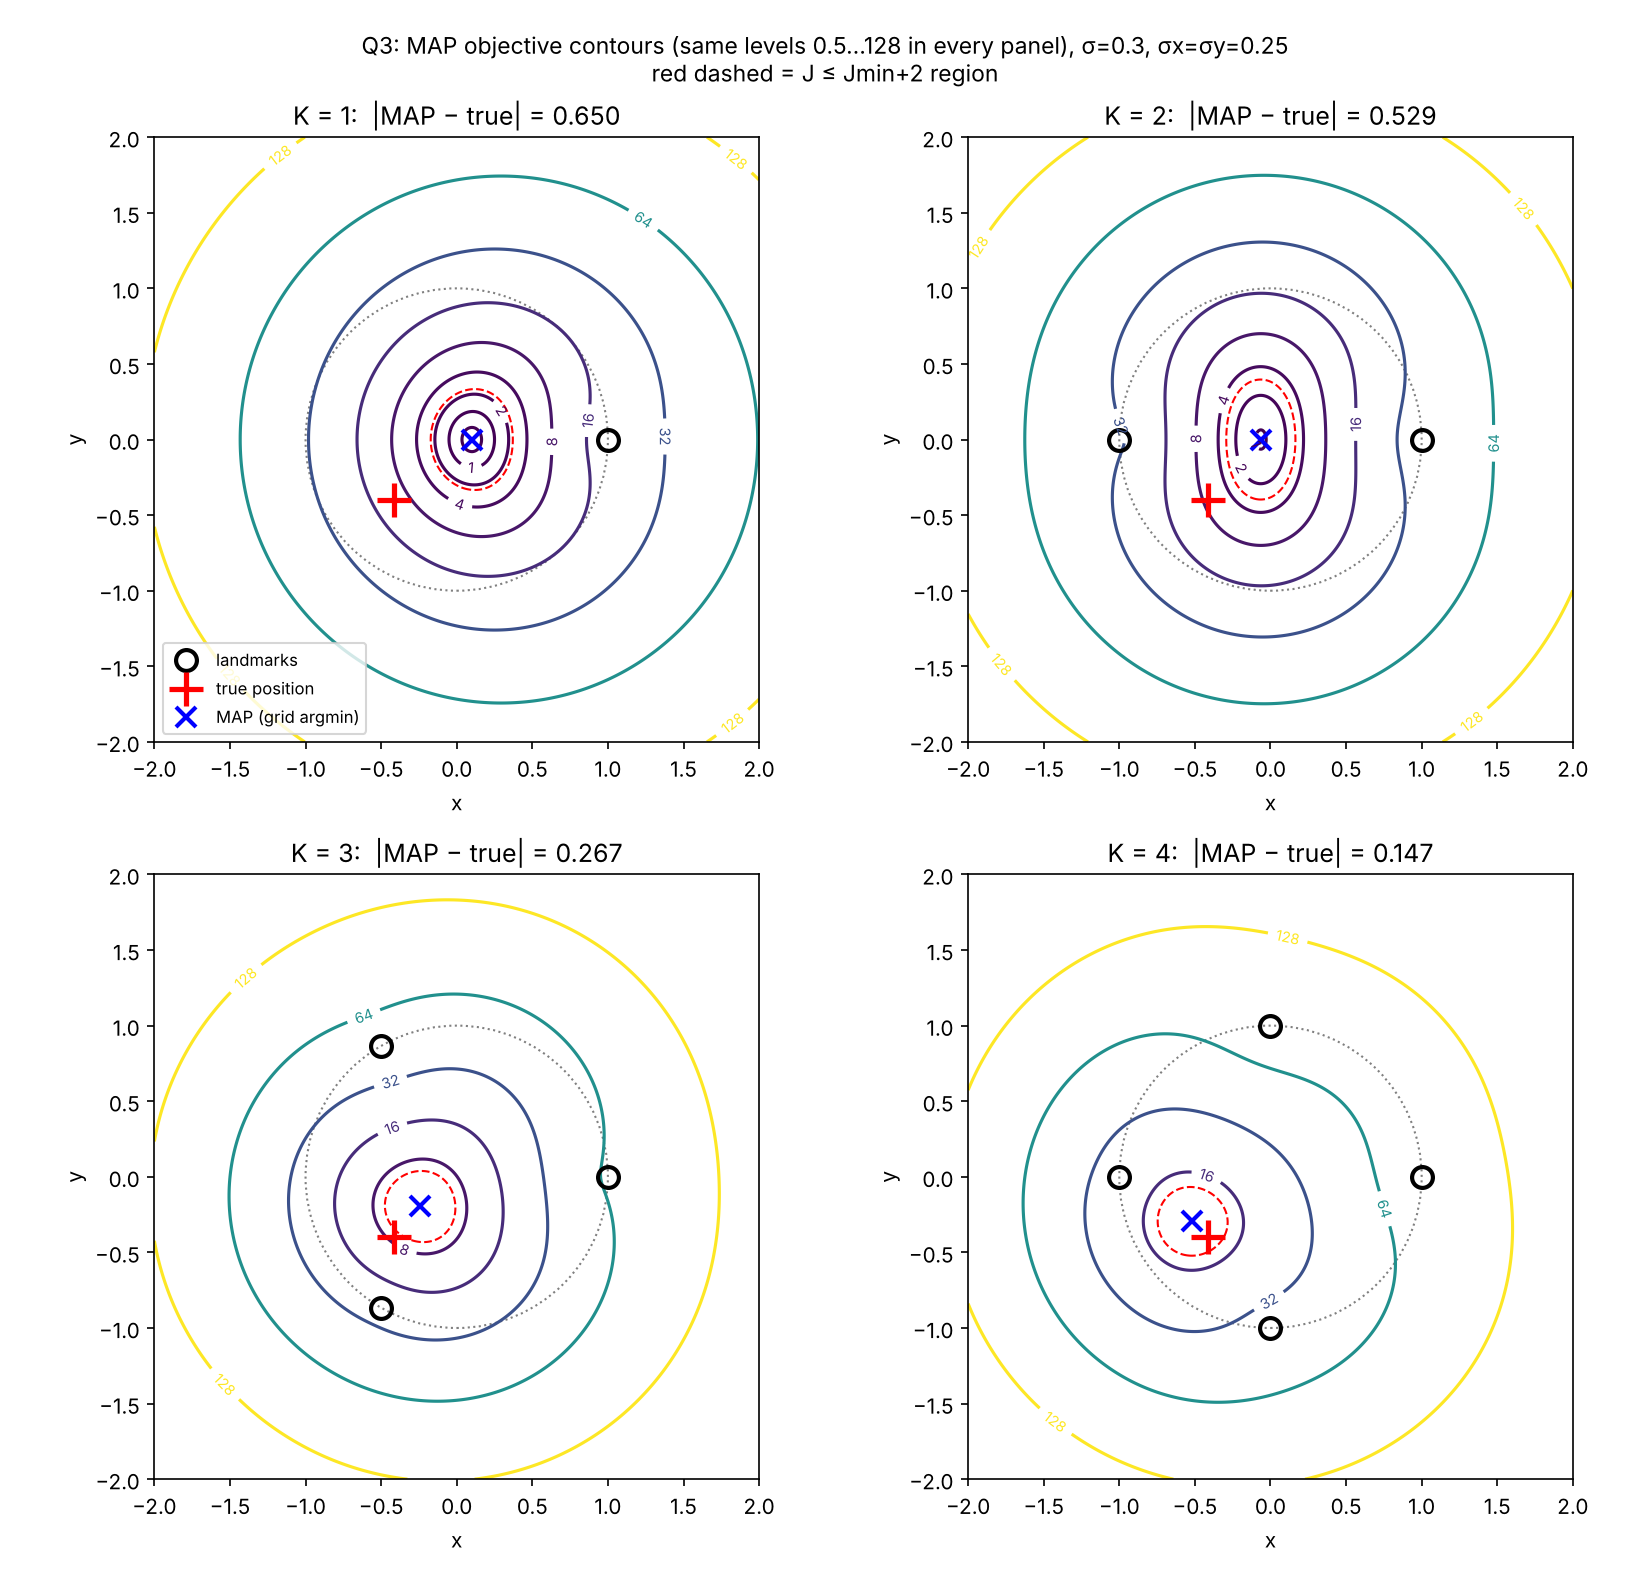
\includegraphics[width=0.92\linewidth]{figs/q3_contours.png}
\caption{MAP objective contours for $K=1,\dots,4$ at identical levels.}
\end{figure}

\begin{table}[H]\centering
\resizebox{\linewidth}{!}{\begin{tabular}{ccccc}\toprule
$K$ & $\hat{\mathbf p}_{MAP}$ & $\|\hat{\mathbf p}_{MAP}-\mathbf p_T\|$ & area of $\{J\le J_{\min}+2\}$ & Monte Carlo mean error / area (500 runs)\\\midrule
1 & $(0.100,\,0.000)$ & 0.650 & 0.287 & 0.558 / 0.311\\
2 & $(-0.065,\,0.000)$ & 0.529 & 0.292 & 0.515 / 0.286\\
3 & $(-0.240,\,-0.195)$ & 0.267 & 0.173 & 0.374 / 0.201\\
4 & $(-0.520,\,-0.295)$ & 0.147 & 0.165 & 0.332 / 0.172\\\bottomrule
\end{tabular}}
\caption{MAP estimates for the plotted realization, plus averages over 500 random true positions and noise draws.}
\end{table}

\subsection*{Discussion}
\begin{itemize}
\item \textbf{$K=1$:} one range only constrains the vehicle to a ring of radius $r_1$ around the landmark; it says nothing about direction. The prior pulls the estimate to the point of that ring nearest the origin, so the MAP lies on the line joining the landmark and the origin, at $(0.10,0)$, far from the truth. Contours are nearly circular and centered near the origin: the prior dominates.
\item \textbf{$K=2$:} the two landmarks $(\pm1,0)$ are collinear with the origin, so both the likelihood and the origin-centered prior are unchanged by $y\to-y$: the two range rings intersect at two mirror points and the data cannot tell them apart. The posterior therefore remains symmetric about the horizontal axis. In this realization its maximum occurs on that axis; in general it need not, and two equally optimal mirrored off-axis estimates can occur, because the symmetric prior cannot distinguish mirrored positions. The contours are elongated vertically (high uncertainty in $y$, good information in $x$).
\item \textbf{$K=3,4$:} three or more non-collinear landmarks triangulate the position uniquely. The innermost contours move off the origin toward the true position (error $0.27$, then $0.15$), and the bowl becomes visibly steeper: at the same contour levels, the curves are more tightly packed, and the low levels (0.5--8) disappear because more measurement terms add to $J$.
\item \textbf{Closer and more certain as $K$ grows.} On average, yes: over 500 runs the mean error falls monotonically from 0.56 to 0.33 and the mean area of the $J\le J_{\min}+2$ region shrinks from 0.31 to 0.17. A single realization need not improve at every step: in the plotted run the error decreases at each $K$, but the region area slightly increases from $K=1$ to $K=2$ (0.287 to 0.292) before shrinking for $K=3,4$. The area is an objective-based proxy for posterior uncertainty, not an exact credible region. More measurements make the likelihood sharper relative to the fixed prior, so the posterior concentrates near the truth. Some residual pull toward the origin remains for all $K$ because the prior ($\sigma_x=\sigma_y=0.25$) is strong compared with the range noise ($\sigma=0.3$); a weaker prior would let the estimate move further toward the data.
\end{itemize}

%=====================================================================
\section*{Question 4 (Duda--Hart--Stork Problem 2.13)}
The conditional risk of action $\alpha_i$ is $R(\alpha_i|\x)=\sum_{j=1}^c\lambda(\alpha_i|\omega_j)P(\omega_j|\x)$.

\textbf{Deciding a class} $\alpha_i$, $i\in\{1,\dots,c\}$: the loss is $0$ when $j=i$ and $\lambda_s$ otherwise, so
\[
R(\alpha_i|\x)=\lambda_s\sum_{j\ne i}P(\omega_j|\x)=\lambda_s\big[1-P(\omega_i|\x)\big].
\]
\textbf{Rejecting} ($\alpha_{c+1}$): the loss is $\lambda_r$ for every true class, so
\[
R(\alpha_{c+1}|\x)=\lambda_r\sum_{j=1}^cP(\omega_j|\x)=\lambda_r .
\]
The Bayes (minimum-risk) rule picks the action with the smallest conditional risk.
\begin{enumerate}
\item Among the $c$ classification actions, $\lambda_s[1-P(\omega_i|\x)]$ is smallest for the class with the largest posterior, so if we classify at all we choose $\omega_i$ with $P(\omega_i|\x)\ge P(\omega_j|\x)$ for all $j$.
\item This best classification beats rejection iff
\[
\lambda_s\big[1-P(\omega_i|\x)\big]\le\lambda_r\iff P(\omega_i|\x)\ge 1-\frac{\lambda_r}{\lambda_s}.
\]
\end{enumerate}
Hence the minimum risk is obtained by deciding $\omega_i$ if $P(\omega_i|\x)\ge P(\omega_j|\x)\ \forall j$ \emph{and} $P(\omega_i|\x)\ge1-\lambda_r/\lambda_s$, and rejecting otherwise. Since the overall risk $R=\int R(\alpha(\x)|\x)p(\x)\,d\x$ is minimized by minimizing the conditional risk at every $\x$, this rule minimizes the total risk. $\blacksquare$

\textbf{If $\lambda_r=0$:} the threshold is $1-0=1$, so we classify only when $P(\omega_i|\x)=1$ (complete certainty) and otherwise reject. Rejection is free, so we always reject whenever there is any chance of error.

\textbf{If $\lambda_r>\lambda_s$:} the threshold $1-\lambda_r/\lambda_s<0$ is satisfied by every posterior, so we never reject; the rule reduces to the ordinary MAP (minimum-error) classifier. Rejecting costs more than even a wrong decision. (More generally, since $\max_iP(\omega_i|\x)\ge1/c$, rejection never occurs once $\lambda_r\ge\frac{c-1}{c}\lambda_s$.)

%=====================================================================
\section*{Question 5}
With 1-of-$K$ coding, $P(\z|\Theta)=\prod_{k=1}^K\theta_k^{z_k}$, with $\theta_k\ge0$, $\sum_k\theta_k=1$. Let $N_k=\sum_{n=1}^Nz_{nk}$ be the number of samples in state $k$ ($\sum_kN_k=N$).

\subsection*{ML estimator}
\[
p(D|\Theta)=\prod_{n=1}^N\prod_{k=1}^K\theta_k^{z_{nk}}=\prod_{k=1}^K\theta_k^{N_k},\qquad
\ln p(D|\Theta)=\sum_{k=1}^KN_k\ln\theta_k .
\]
Maximize subject to $\sum_k\theta_k=1$ with a Lagrange multiplier:
\[
\mathcal L=\sum_kN_k\ln\theta_k+\lambda\Big(1-\sum_k\theta_k\Big),\qquad
\frac{\partial\mathcal L}{\partial\theta_k}=\frac{N_k}{\theta_k}-\lambda=0\Rightarrow\theta_k=\frac{N_k}{\lambda}.
\]
Summing over $k$: $1=\sum_kN_k/\lambda=N/\lambda\Rightarrow\lambda=N$. Thus
\[
\boxed{\hat\theta_k^{ML}=\frac{N_k}{N}=\frac1N\sum_{n=1}^Nz_{nk},\qquad\hat\Theta_{ML}=\frac1N\sum_{n=1}^N\z_n,}
\]
the relative frequency of each state. It is the global maximum because $\sum_kN_k\ln\theta_k$ is concave and the constraint set is convex.

\subsection*{MAP estimator with Dirichlet prior}
\[
p(\Theta|D)\propto p(D|\Theta)p(\Theta|\alpha)\propto\prod_{k=1}^K\theta_k^{N_k}\cdot\prod_{k=1}^K\theta_k^{\alpha_k-1}=\prod_{k=1}^K\theta_k^{N_k+\alpha_k-1}
\]
(the posterior is again Dirichlet, with parameters $N_k+\alpha_k$; $B(\alpha)$ does not depend on $\Theta$ and is dropped). Maximizing $\sum_k(N_k+\alpha_k-1)\ln\theta_k$ subject to $\sum_k\theta_k=1$ exactly as above gives $\theta_k=(N_k+\alpha_k-1)/\lambda$ with $\lambda=\sum_k(N_k+\alpha_k-1)=N+\sum_k\alpha_k-K$:
\[
\boxed{\hat\theta_k^{MAP}=\frac{N_k+\alpha_k-1}{N+\sum_{j=1}^K\alpha_j-K}.}
\]
The stationarity derivation assumes an interior maximum, which holds when $N_k+\alpha_k>1$ for every $k$ (for example, all $\alpha_k>1$); the objective is then strictly concave on the simplex. Note that $\alpha_k\ge1$ is not enough: with $\alpha_k=1$ and $N_k=0$, $\theta_k$ has exponent $0$, so the posterior does not increase with $\theta_k$ and the maximum sits on the boundary at $\hat\theta_k=0$. The formula still returns this value (provided some other $N_j+\alpha_j>1$), but it is a boundary solution, not a stationary point. If some $N_k+\alpha_k<1$, the posterior density is unbounded as $\theta_k\to0$, so no finite maximum exists and the MAP estimate is not well defined.

\textbf{Interpretation.} $\alpha_k-1$ acts as a pseudo-count added to the observed count of state $k$. With a uniform prior ($\alpha_k=1$) the MAP equals the ML estimate; $\alpha_k=2$ gives Laplace (add-one) smoothing, which avoids zero probabilities for unseen states; and as $N\to\infty$ the data dominate and $\hat\Theta_{MAP}\to\hat\Theta_{ML}$.

%=====================================================================
\section*{Acknowledgement of resources and AI use}
\textbf{[Review and edit this statement so that it accurately describes how you used these tools before submitting.]}
I used Claude (Anthropic, model Claude Opus 5.5, via claude.ai, October 25, 2026) as a coding and writing assistant for this assignment. It helped write the Python implementations in the Appendix, run the experiments, produce the figures, draft the derivations for Questions 1--5, and typeset this report. I reviewed the derivations and results. The data generator for Question 2 is the course-provided \texttt{hw2q2.py}. Libraries used: NumPy, SciPy (\texttt{scipy.stats.multivariate\_normal}, \texttt{scipy.optimize.minimize}), Matplotlib. Question 4 is Problem 2.13 from R.~O.~Duda, P.~E.~Hart, D.~G.~Stork, \emph{Pattern Classification}, 2nd ed., Wiley, 2001.

%=====================================================================
\newpage
\section*{Appendix: Code}
\subsection*{q1.py}
\VerbatimInput[fontsize=\scriptsize,frame=single]{q1.py}
\subsection*{q2.py}
\VerbatimInput[fontsize=\scriptsize,frame=single]{q2.py}
\subsection*{q3.py}
\VerbatimInput[fontsize=\scriptsize,frame=single]{q3.py}
\end{document}
